%1) Spécification de l’environnement 
%        2) Specification du logiciel : Generation Controlée
%                2.1 Fonctionnalité
%                2.2 Decompo fonctionnelle
%        3) Conception fonctionnelle
%        4) Definition de la réalisation 
%        5) Réalisation 
%        6) Tests


\chapter{Générateur de tâches}
	\label{chap:1}
	
	\section{Spécification de l’environnement}
	Lorsque le programme est lancé, l’utilisateur doit choisir le mode de génération. Il rentre les données nécessaires au bon déroulement du mode. Le programme crée un fichier qui contient le résultat de la génération de tâches.


	\section{Spécification du logiciel}

		\subsection{Explication du choix du langage}
	
			\label{sec:langage}
			Nous avons opté pour le langage C++ pour réaliser ce projet car celui-ci possède un certain nombre d'avantages. Il s'agit d'un langage orienté objet très utilisé dans le monde et de nombreux outils libres sont disponibles pour l'utiliser (comme GCC pour la compilation par exemple). De plus, la documentation correspondante est très facilement accessible dans la littérature ou sur le web.
		
			Bien que le travail qui nous a été demandé ne requiert pas la maîtrise d'une programmation bas niveau, le langage C++ nous apparait en cohérence avec le thème abordé par le projet (les systèmes temps réel embarqués).

		\subsection{Fonctionnalités}

			\Huge
			A mettre : un petit schéma comme on a fait au premier TP qui montre le lien entre les différents modules
			\normalsize
		    
			\subsubsection{Choix du mode}
				Dans ce premier module, on choisit le mode d’utilisation du logiciel en fonction de ce que souhaite l’utilisateur. Pour cela, il peut soit renseigner sous forme d’arguments les différentes données, soit en sélectionnant dans le menu ses préférences. \\

				Parmi les choix qui lui sont offerts, on retrouve les cas présentés dans le sujet du projet (génération aléatoire ou contrôlée et tâches périodiques ou non) mais aussi la possibilité de renseigner un fichier contenant déjà toutes les informations sur les tâches. Dans le premier cas, l’utilisateur devra renseigner ensuite le nombre de tâches concernées tandis que dans l’autre cas, le fichier ne sera pas interprété et ce programme s’arrêtera.


			\subsubsection{Génération aléatoire de tâches}
				Le premier type de génération permet de générer automatiquement des tâches. L'utilisateur devra renseigner le nombre de tâches périodiques et apériodiques à générer ainsi que le pourcentage d'utilisation du CPU. Ceci permet de générer des fichiers de test aléatoire qui seront visualisable par la suite.\\
				Lors de la génération, le système calcule les différentes valeurs caractéristiques des tâches 

			\subsubsection{Génération contrôlée de tâches}
				Le deuxième type de génération fait appel à l'utilisateur pour renseigner chacune des valeurs de chaque tâche. De cette manière, l'utilisateur va pouvoir tester plus facilement des cas spécifiques et donc observer de manière plus précise le fonctionnement de l'ordonnanceur par la suite. \\
				Lors de la génération, pour toutes les tâches périodiques il devra renseigner les Ci, Pi et Di, c'est-à-dire respectivement les durées d'exécution maximales, les périodes d'activation et le délai critique). Dans le cas où il y a aussi des tâches apériodiques, il devra renseigner aussi ri (la date de réveil) et Ci.

			\subsubsection{Écriture dans un fichier}
				Ce module a pour fonction d’écrire dans un fichier les données contenues dans un flux (= stream)  et calculées à partir des deux modules précédents de génération. L’intérêt de séparer ces fonctions est double : il est plus pratique de factoriser le code à travers une seule fonction d’écriture appelée par les différentes générations et cela facilite la maintenance.


		\subsection{Décomposition fonctionnelle}
			Une classe par type de génération 


	\section{Conception fonctionnelle}

		\subsection{Choix du mode}
			\paragraph{Pré-condition :} Le programme vient d’être lancé.
			\paragraph{Post-condition :} Un choix valide a été effectué.
			\paragraph{Objectif :} Permettre de choisir entre la génération aléatoire et la génération controlée.
			\paragraph{Algo :}
			\begin{verbatim} 
	Entrée : Int choix
	Sortie :  -

Si (choix == 1 ) Alors
   Lancer la génération controlée
Sinon
   Si (choix == 2) Alors
	  Lancer la génération aléatoire 
   Sinon
	  Si (choix == 3) Alors
	     Quitter le programme
	  Sinon
	     Afficher erreur de choix 
	  FinSi
   FinSi
FinSi
		\end{verbatim} 

	\newpage
	\subsection{Génération Aléatoire}
		\paragraph{Pré-condition :} La génération aléatoire a été choisie.
		\paragraph{Post-condition :} Toutes les valeurs caractéristiques des tâches ont été générées en accord avec le paramétrage de l’utilisateur.


		\paragraph{Objectif :} Générer aléatoirement les caractéristiques (Ci,Pi,Di) d’un nombre de tâches (determiné par l’utilisateur) en accord avec un facteur d’utilisation du processeur (déterminé lui aussi par l’utilisateur).
		Ex : pour trois taches et facteur = 75\% \\ 


		    Tirage aléatoire de trois nombres ( 35, 25, 15) dont la somme vaut 75. \\
		    Ces nombres représentent le rapport Ci/Pi dans la formule  \\
		    Il faut ensuite donner une valeur à Ci et Pi. Pour cela, on trouve le pgcd du nombre et de 100. Pour C1/P1 = 35, on obtient 5.  on affecte à C1 $\leftarrow$ 35/5 et à P1 $\leftarrow$ 100/5 , on obtient donc C1 = 7 et P1 = 20. On considère, dans ce programme que Pi = Di. \\
		    
		    On obtient donc dans cette exemple :  \\
		    T1(7,20,20) \\
		    T2(1,4,4) \\
		    T3(3,20,20) \\

		    Toutes les données sont stockées dans 3 tableaux (un pour les Ci, un pour Pi, un pour Di). 

		\paragraph{Algo :}
			\begin{verbatim}
Entrée: Int nbTaches, Int factUtProcesseur
Sortie : 3 Tableaux d’Int (pour les valeurs de Ci, Pi, Di). 
indice du tableau = numéro de la tâche - 1..

TabCi[ nbTaches ], TabPi[ nbTaches ], TabDi[ nbTaches ]
nbTachesRestantes = nbTaches - 1
nbMax = factUtProcessus 

/*
On calcule la valeur maximale que peut prendre le nombre tiré aléatoirement :
maximum = Up - somme des Ci/Pi précédents - nombre de taches restantes
Ensuite, on tire au hasard une valeur allant de 1 à cette valeur maximale.
Exemple : maxT1 = 75 - 0 - 2
	    randT1 = 32 (valeur calculée avec le pseudo-hasard)
	    maxT2 = 75 - 32 - 1
	    randT2 = 18
	    maxT3 = 75 - (32 + 18) - 0
	    randT3 = 25
Pour résumer, on obtient ici les Ci/Pi : 32, 18 et 25
*/


Pour i allant de 0 à (nbTaches - 1)
   nbMaxLimite = nbMax - nbTachesRestantes
   // le nombre aléatoire correspond à (Ci/Pi)
   nbAleatoire = nombre Aleatoire entre 1 et ce nombre maximum


   // On calcule et stocke la valeur des Ci, Pi et Di dans 3 tableaux distincts
   tabCi[i] = nb\_genere / pgcd(nb\_genere,100)
   tabPi[i] =100 / pgcd(nb\_genere,100)
   tabCi[i] = 100 / pgcd(nb\_genere,100)
	        
   /* On abaisse ensuite la limite pour le prochain tirage aléatoire afin de ne jamais dépasser la valeur de Up. */
   limite\_maj = limite\_maj - nb\_genere
Fin du pour

// Pour la dernière tâche, on ne génère pas de valeur. On prend ce qu’il reste.
nb\_genere = limite\_maj
tabCi[ nbTaches - 1 ] = nb\_genere / pgcd(nb\_genere,100)
tabPi[ nbTaches - 1 ] =100 / pgcd(nb\_genere,100)
tabCi[ nbTaches - 1 ] = 100 / pgcd(nb\_genere,100)
			\end{verbatim}

	\subsection{Generation Controlée}  
		\paragraph{Pré-condition :} La génération controlée a été choisie.
		\paragraph{Post-condition :} Toutes les valeurs caractéristiques des tâches ont été générées en accord avec le paramétrage de l’utilisateur.
		\paragraph{Objectif :} Permettre à l’utilisateur de générer des tâches périodiques ou apériodiques en renseignant les différentes caractéristiques de chacune des tâches (Ci, Pi, Di).
		\paragraph{Algo :} 
			\begin{verbatim}
Entrée : Int nbTaches
Sortie :  3 Tableaux d’Int (pour les valeurs de Ci, Pi, Di). 
indice du tableau = numéro de la tâche - 1 .


TabCi[ nbTaches ], TabPi[ nbTaches ], TabDi[ nbTaches ]
		
Pour i allant de 0 à (nbTaches - 1)
	// on demande à l’utilisateur de renseigner les différentes valeurs ...
	lire(Ci)
	lire(Pi)
	lire(Di)        
	// … et on les insére dans les tableaux respectifs
	tabCi[ i ] = Ci
	tabPi[ i ] = Pi
	tabDi[ i ] = Di
fin pour
			\end{verbatim}

	\subsection{Ecriture du résultat obtenu}
		\paragraph{Pré-condition :} La génération (qu'elle soit contrôlée ou non) envoie un outputstream contenant les chaînes de caractère à écrire dans un fichier.
		\paragraph{Post-condition :} L'écriture s'est bien déroulée : le fichier contient bien la chaîne.
		\paragraph{Objectif :} Enregistrer les données générées par le module précédent de manière pérenne dans un fichier.
		\paragraph{Algo :}
		\Huge
		TODO
		\normalsize

\section{Définition de la réalisation}
	\Huge
	TODO
	\normalsize

\section{Réalisation}
	\subsection{Répartition des tâches}

\section{Tests}



\chapter{Simulateur d'ordonnanceur}
	\section{Spécification de l’environnement}
		Le programme final devra pouvoir être exécutable en ligne de commande.\\
		
		En entrée : le nom du fichier contenant le jeu de tâches périodiques et apériodiques pour lesquelles on veut simuler l'ordonnancement.\\
		
		En sortie : un ou plusieurs fichiers .ktr utilisable avec l'outil Kiwi\footnote{\Huge TODO présenter kiwi vite fait} et contenant la séquence d'ordonnancement. Le programme affichera également quelques résultats via la sortie standard.\\
		
		Afin de faciliter la prise en main du programme, on proposera un menu succint présentant les différentes fonctionnalités qui s'offrent à l'utilisateur.
	
	\section{Specification du logiciel}
		Pour les mêmes raisons que celles décrites dans le Chapitre \ref{sec:langage}, le langage utilisé est le C++.

		\subsection{Fonctionnalité}
			\begin{figure}
				\centering
				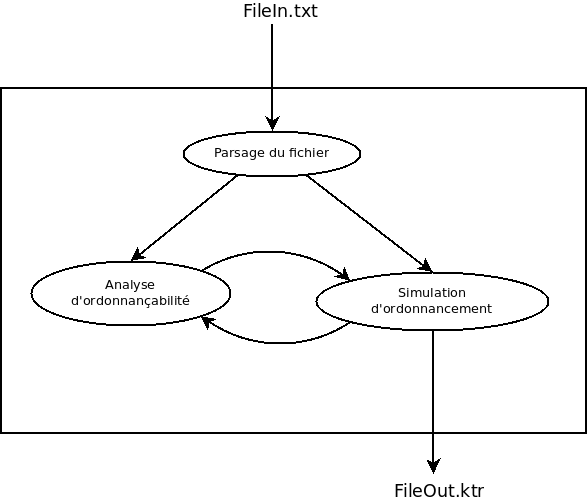
\includegraphics[scale=0.55]{ordo_fct_diag.png}
				\caption{Diagramme des fonctionnalités}
			\end{figure}
			\FloatBarrier
			
			\subsubsection{Parsage du fichier d'entrée}
				Vérification de la syntaxe avec expression régulière + enregistrement des tâches et de leurs paramètres dans un modèle.
			
			\subsubsection{Analyse d'ordonnançabilité}
				On fait tous les calculs en même temps :
				\begin{itemize}
					\item Condition nécessaire pour l'ordonnançabilité du jeu de tâche avec RM ;
					\item Condition suffisante avec RM ;
					\item Condition suffisante et nécessaire avec EDF.
				\end{itemize}
			
			\subsubsection{Simulation d'ordonnancement}
			
		\subsection{Decomposition fonctionnelle}

	\section{Conception fonctionnelle}
	
		\subsection{Analyse du fichier d'entrée}
				\paragraph{Post-condition :} 
				\paragraph{Objectif :} 
				\paragraph{Algo :} 
					\begin{verbatim}
ALGO TODO
					\end{verbatim}
		
		
		\subsection{Analyse d'ordonnançabilité}
			
			\subsubsection{Condition nécessaire RM}
				\paragraph{Pré-condition :} n représente le nombre de tâches périodiques
				\paragraph{Post-condition :} 
				\paragraph{Objectif :} Vérifier les conditions d'ordonnançabilité nécessaires de l'algorithme RM 
				\paragraph{Algo :} 
					\begin{lstlisting}
U = 0
					
Pour i de 0 \'a n faire
	U = U + Ci/Pi
Finpour		

Si U <= 1.0 alors
	afficher("On ne peut rien conclure")
Sinon
	afficher("Non-ordonnan\c{c}able")
Finsi
					\end{lstlisting}
			
			\subsubsection{Condition suffisante RM}
				\paragraph{Pré-condition :} n représente le nombre de tâches périodiques
				\paragraph{Post-condition :} 
				\paragraph{Objectif :} 
				\paragraph{Algo :} 
					\begin{lstlisting}
U = 0
UBoundRM =  $n * (2^{(1.0 / n)} - 1)$
					
Pour i de 0 \'a n faire
	U = U + Ci/Pi
Finpour

Si U <= UBoundRM alors
	afficher("Ordonnan\c{c}able")
Sinon
	afficher("On ne peut rien conclure")
Finsi
					\end{lstlisting}
			
			\subsubsection{Condition nécessaire et suffisante EDF}
				\paragraph{Post-condition :} 
				\paragraph{Objectif :} 
				\paragraph{Algo :} 
					\begin{lstlisting}
ALGO TODO
					\end{lstlisting}
					
			\subsubsection{Condition nécessaire et suffisante EDF-TBS}
				\paragraph{Post-condition :} 
				\paragraph{Objectif :} 
				\paragraph{Algo :} 
					\begin{lstlisting}
ALGO TODO
					\end{lstlisting}
	
		\subsection{Simulation d'ordonnancement}
			Le simulateur d'ordonnancement est découpé en deux algorithmes principaux :
			\begin{itemize}
				\item RM ;
				\item EDF.
			\end{itemize}
			
			Nous avons en premier lieu commencé par développer ces deux algorithmes sans tenir compte des tâches périodiques dans le but ensuite de les "patcher" avec nos algorithmes d'ordonnancement des tâches apériodiques (BG et TBS).
			
			\subsubsection{Rate Monotonic}
				\paragraph{Pré-condition :} 
				\paragraph{Post-condition :} 
				\paragraph{Objectif :} 
				\paragraph{Algo :} 
					\begin{verbatim}
Entrée : 
Sortie :  


init_context()
int t := 0
int task_executed := -1

tant que (t < getHyperPeriode())
	
    Booleen need_to_poll = poll_needed()
	
    si(need_to_poll)
        
        TODO : ALGO RM
        
    fsi
	
    maj_context()
    t++
	
fin tant que
					\end{verbatim}
					
					
			\subsubsection{Earliest Deadline First}
			
				\paragraph{Pré-condition :} 
				\paragraph{Post-condition :} 
				\paragraph{Objectif :} 
				\paragraph{Algo :} 
					\begin{verbatim}
Entrée : 
Sortie :  


init_context()
int t := 0
int task_executed := -1

tant que (t < getHyperPeriode())
	
	Booleen need_to_poll = poll_needed()
	
	si(need_to_poll)
		
		TODO : ALGO EDF
		
	fsi
	
	maj_context()
	t++
	
fin tant que
					\end{verbatim}
				

	\section{Définition de la réalisation}

	\section{Réalisation}

	\section{Tests}

